\documentclass{article}
 \usepackage{graphicx} 
 \usepackage{amsfonts}
\usepackage{amsmath}
\usepackage{calrsfs}
\usepackage[T1]{fontenc}
\date{}
 \usepackage[colorlinks,urlcolor=blue]{hyperref} 
  \usepackage[left=1.2in,right=1in,top=1in,bottom=.8in]{geometry}
 \date{}
 \title{Devoir personnel}
\begin{document}
\maketitle

\begin{figure}
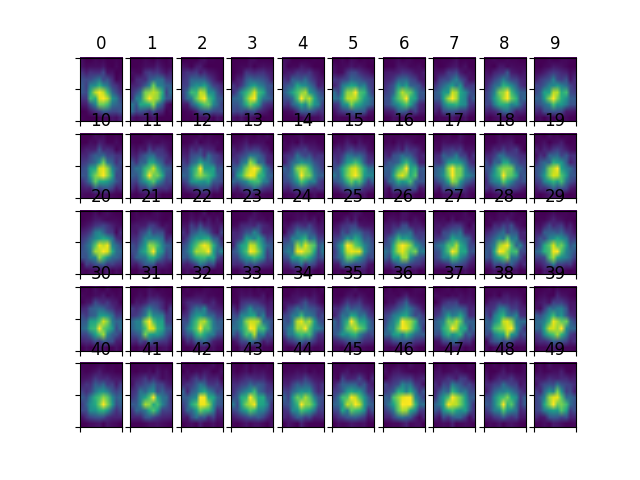
\includegraphics[scale=1]{visu_feature.png}
\end{figure}

\clearpage
\begin{figure}
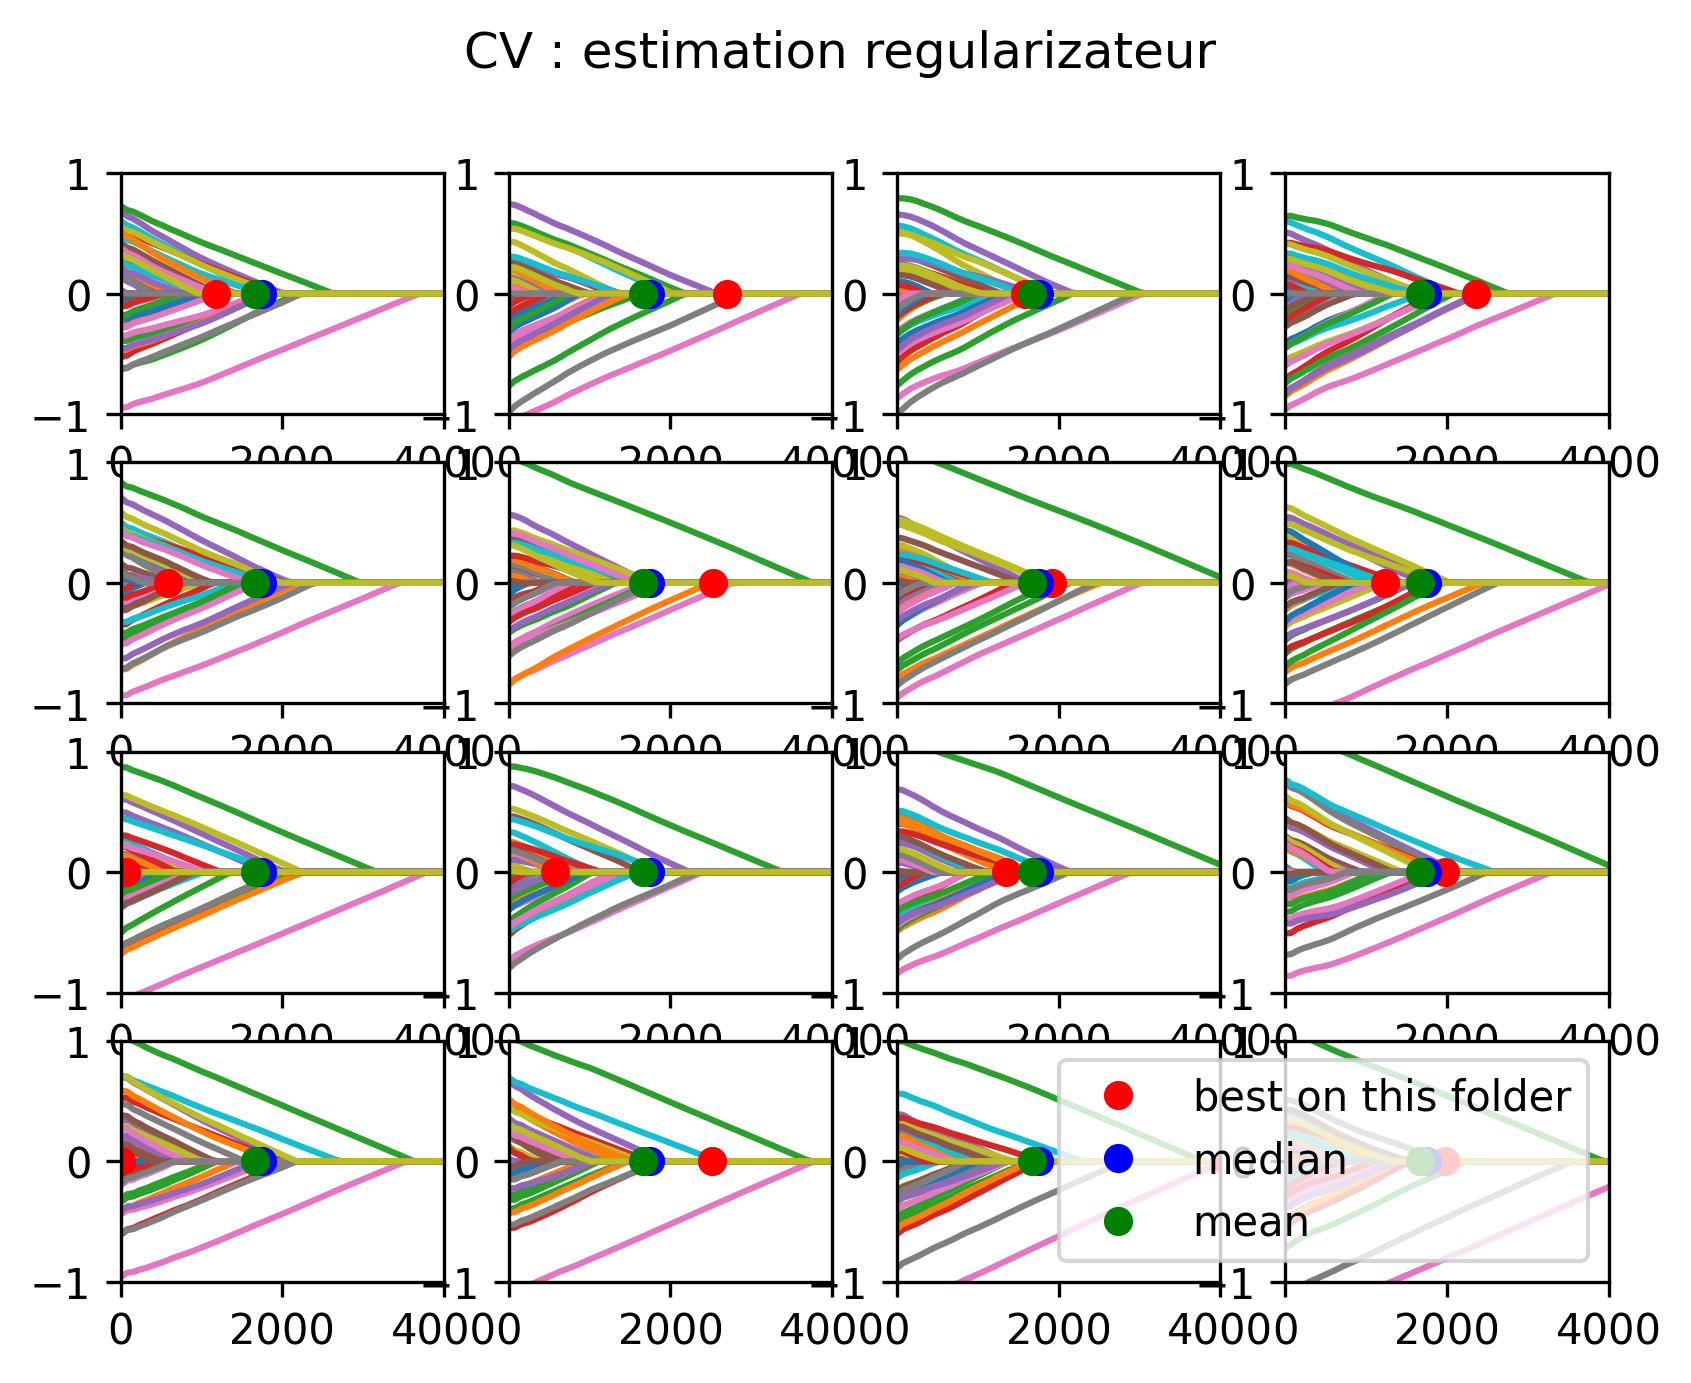
\includegraphics[scale=1]{cv_reg.png}
\end{figure}
\clearpage

\begin{figure}
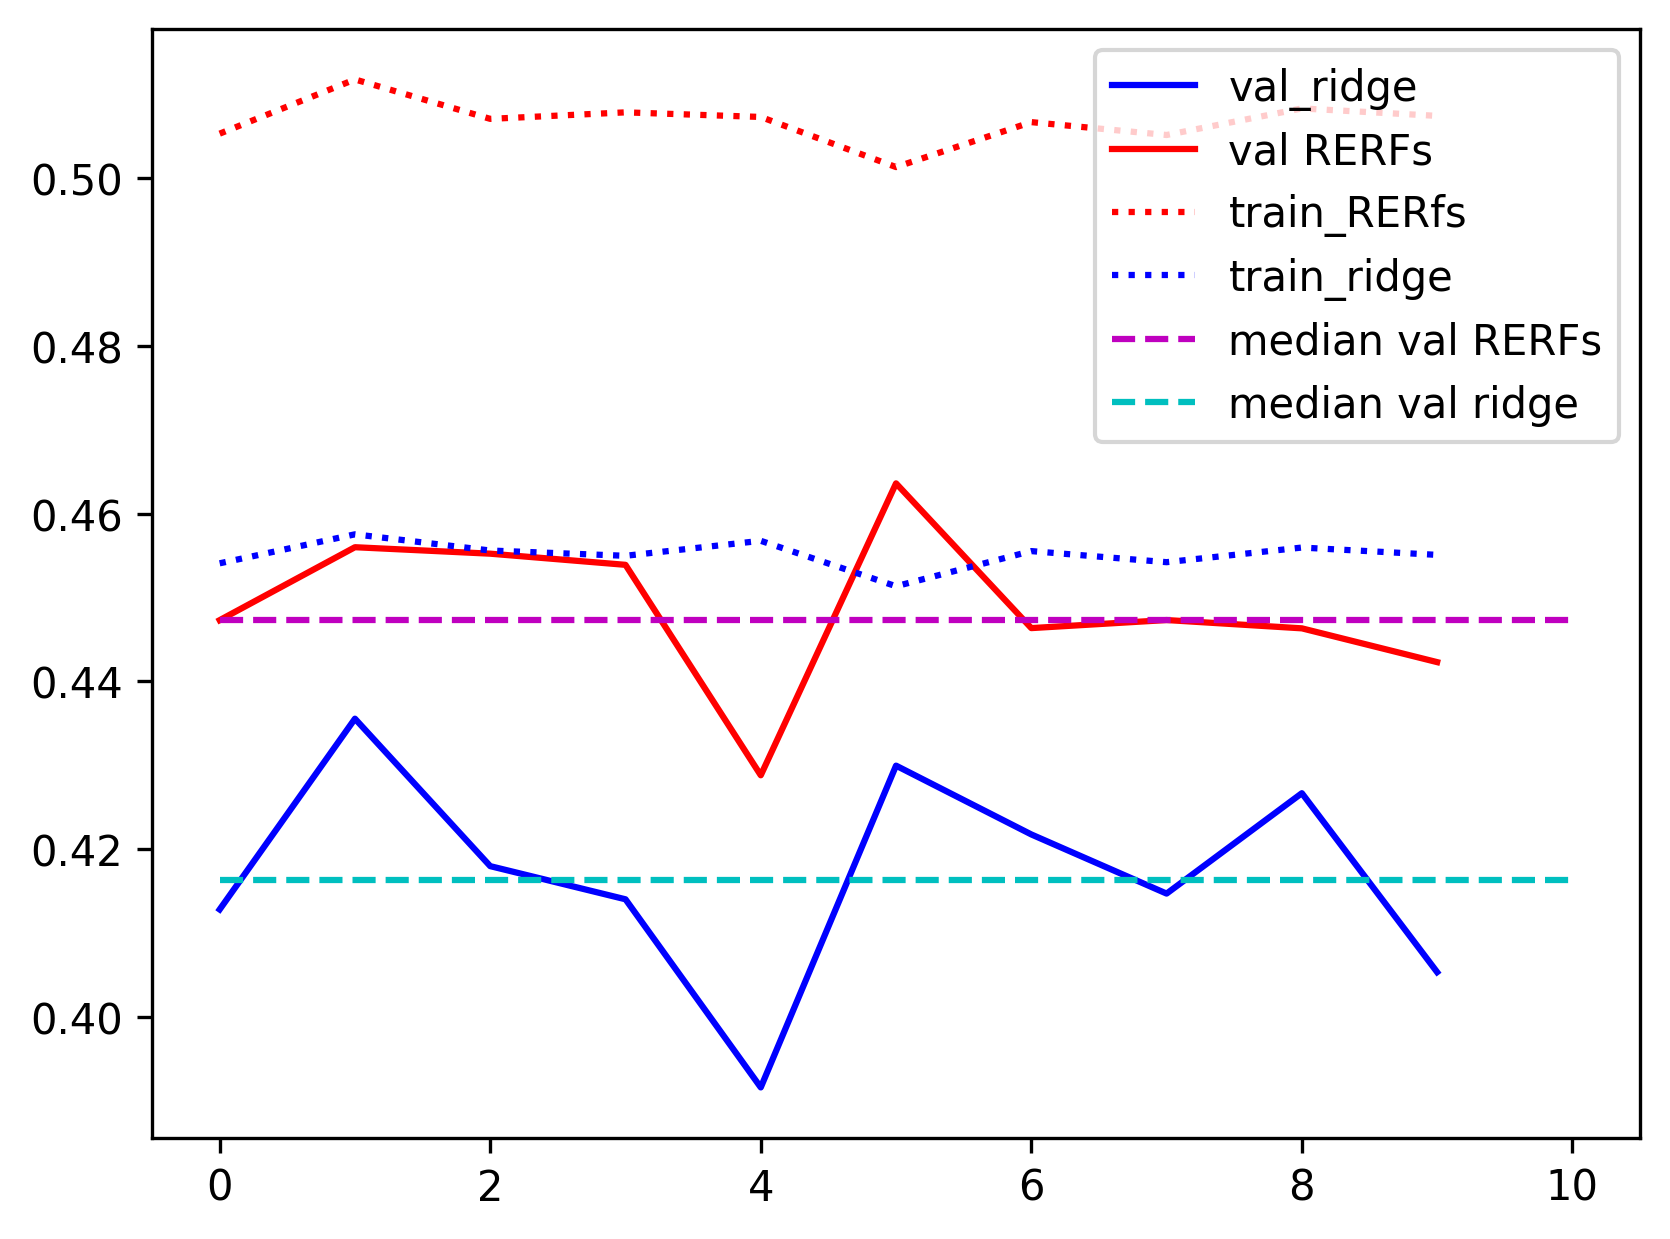
\includegraphics[scale=1]{compare.png}
\end{figure}


\clearpage
\begin{figure}
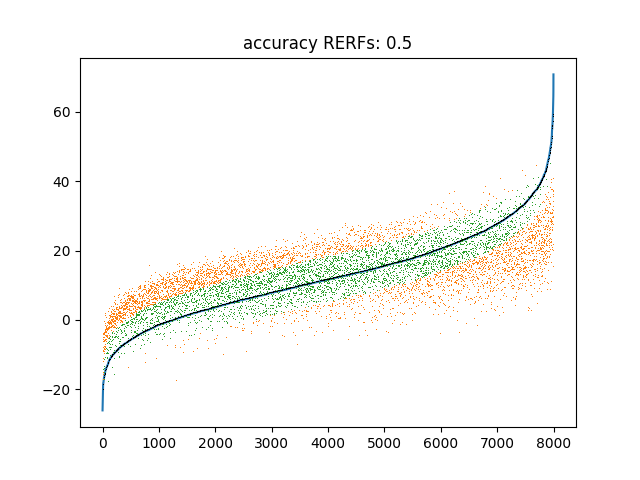
\includegraphics[scale=0.5]{pred_RERFsvs_true.png}
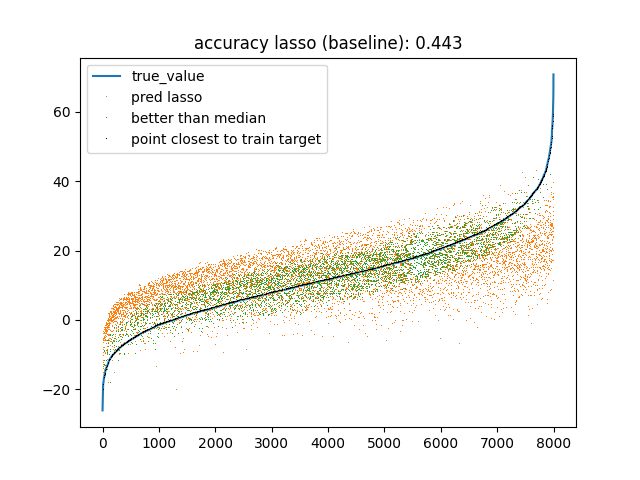
\includegraphics[scale=0.5]{pred_lasso_vs_true.png}
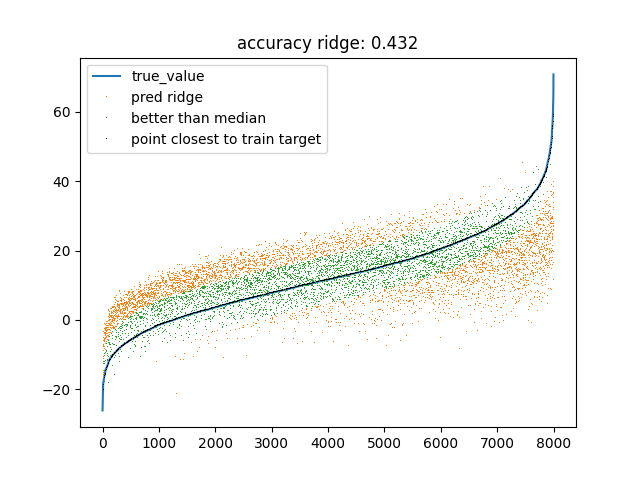
\includegraphics[scale=0.5]{pred_ridge_vs_true.png}
\end{figure}

\newpage


\begin{figure}
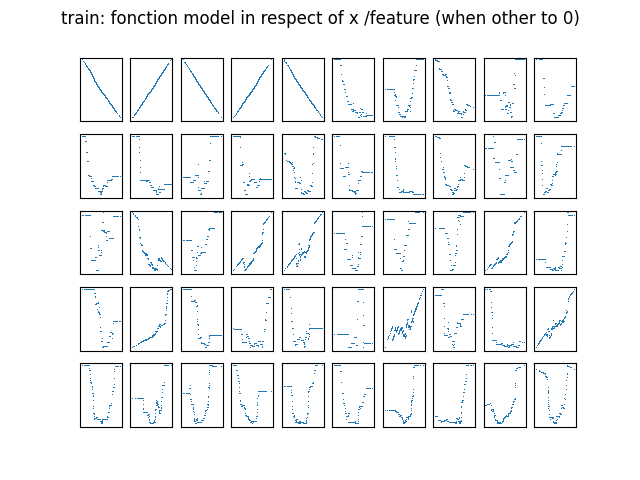
\includegraphics[scale=1]{train_affichage_fonction.png}
\end{figure}

\newpage

\begin{figure}
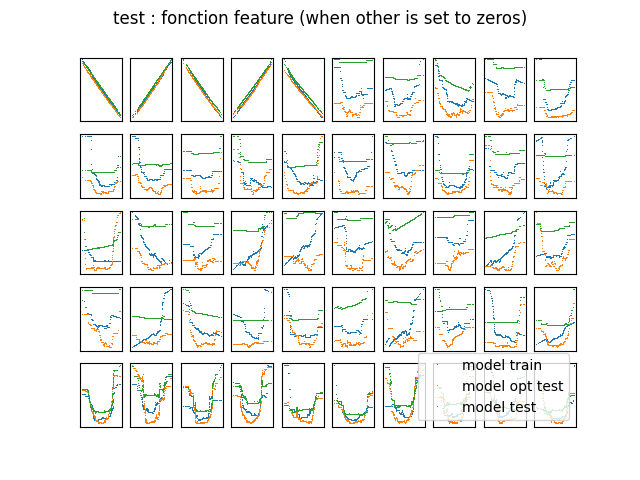
\includegraphics[scale=1]{test_affichage_fonction.png}
\end{figure}

\newpage

\begin{figure}
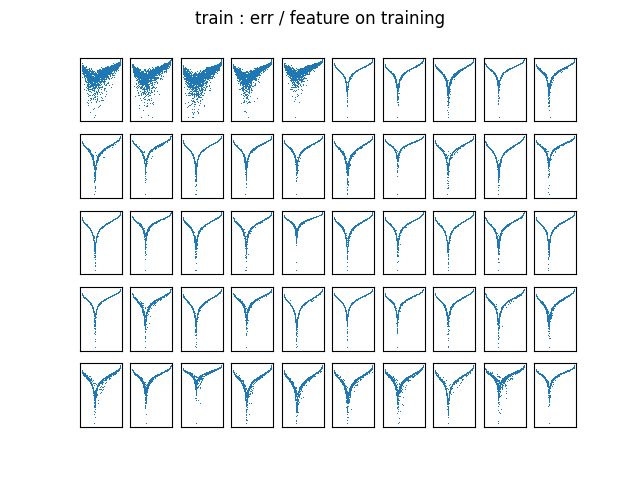
\includegraphics[scale=1]{train_error_par_feature.png}
\end{figure}

\newpage

\newpage

\begin{figure}
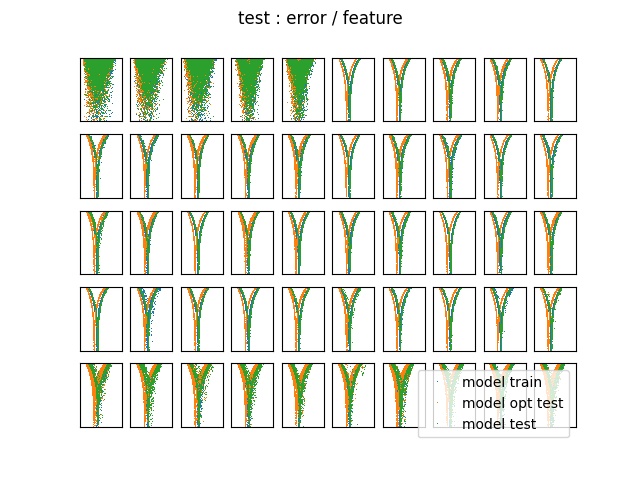
\includegraphics[scale=1]{test_error_par_feature.png}
\end{figure}

\newpage


\begin{figure}
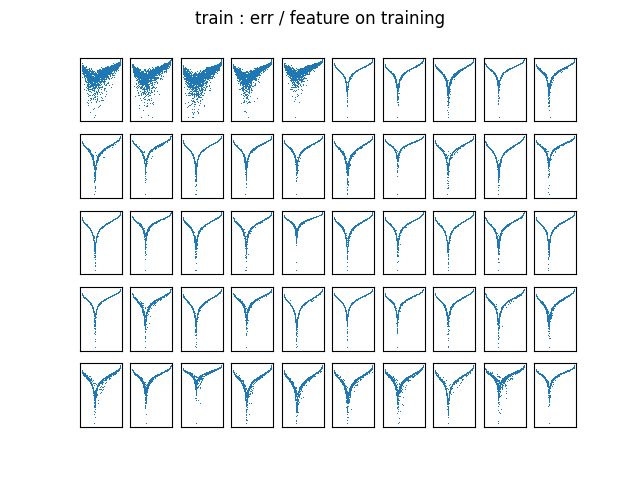
\includegraphics[scale=1]{train_error_par_feature.png}
\end{figure}

\newpage

\begin{figure}
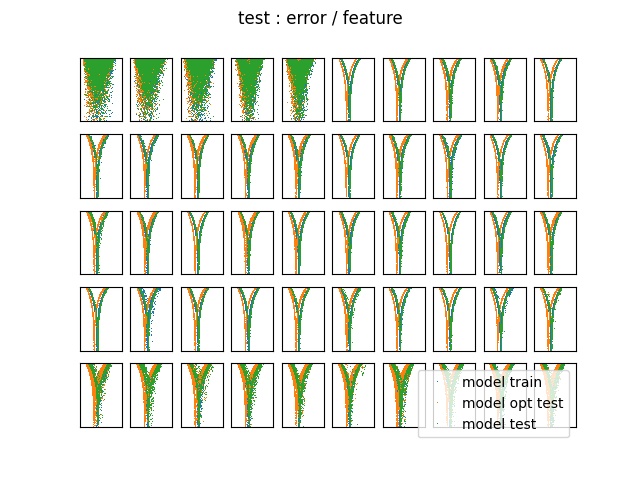
\includegraphics[scale=1]{test_error_par_feature.png}
\end{figure}

\newpage

\begin{figure}
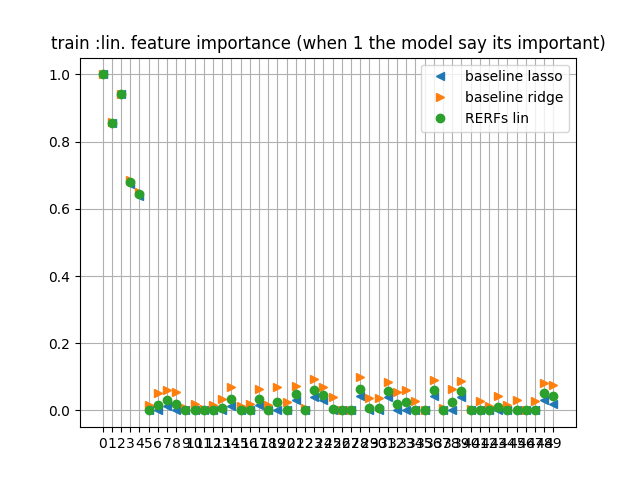
\includegraphics[scale=0.7]{train_linear_feature_importance.png}

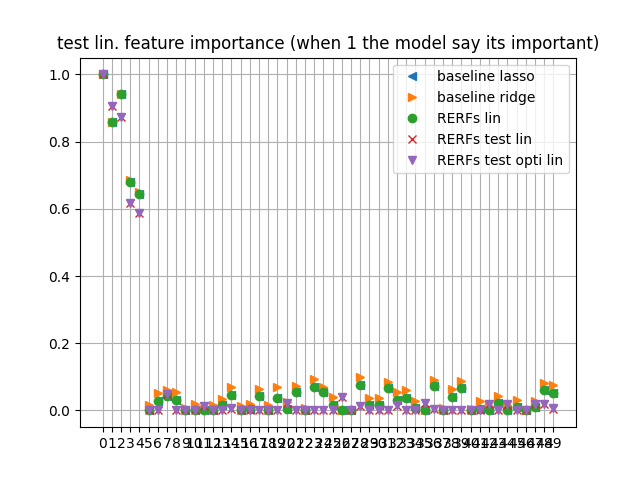
\includegraphics[scale=0.7]{test_linear_feature_importance.png}
\end{figure}

\newpage

\begin{figure}
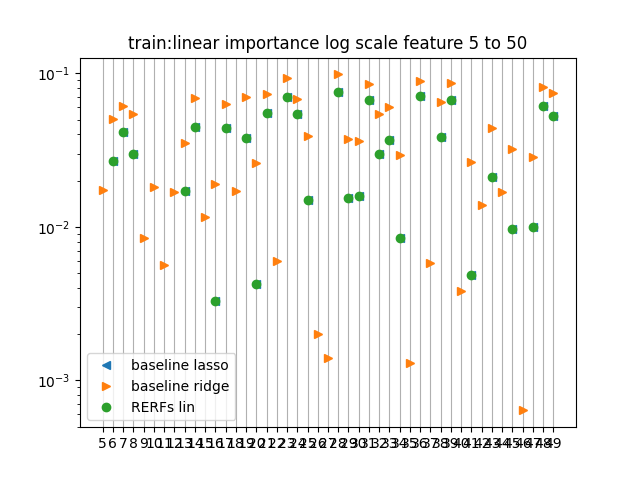
\includegraphics[scale=0.7]{train_linear_feature_importance2.png}

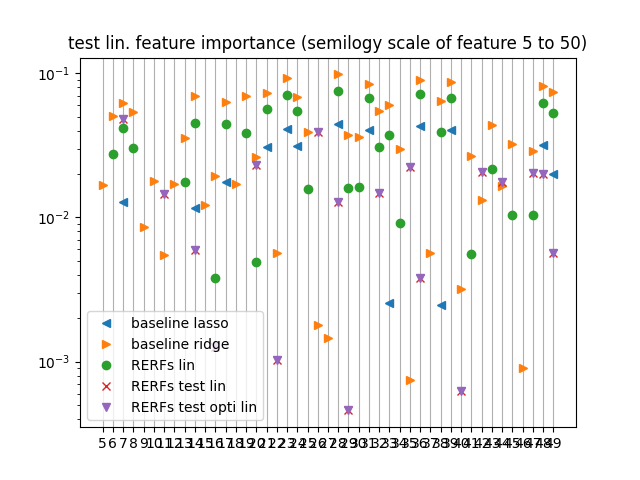
\includegraphics[scale=0.7]{test_linear_feature_importance2.png}
\end{figure}

\newpage
\begin{figure}
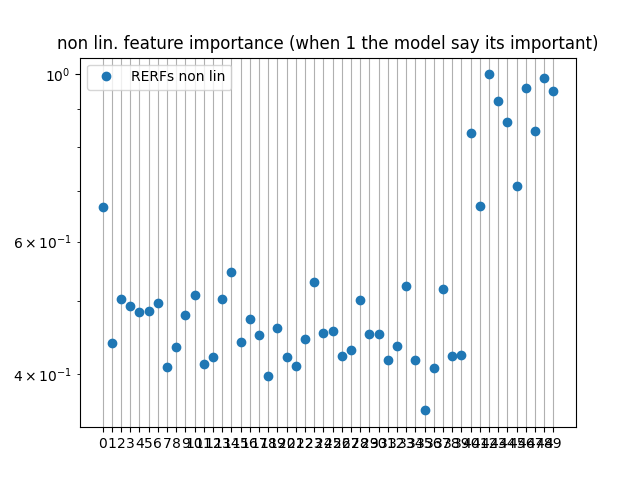
\includegraphics[scale=0.7]{train_non_linear_feature_importance.png}

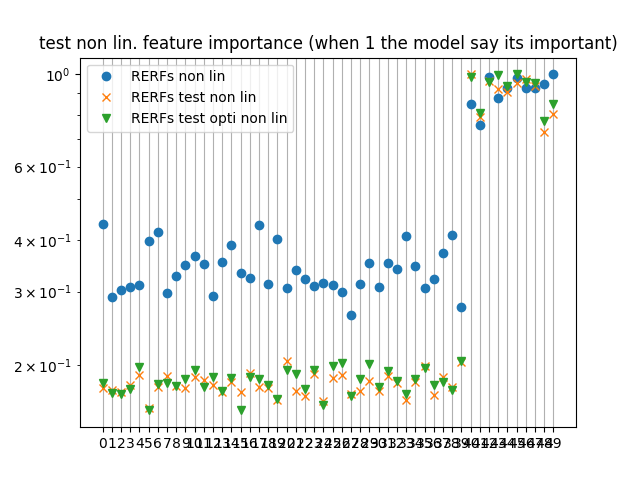
\includegraphics[scale=0.7]{test_non_linear_feature_importance.png}
\end{figure}


\end{document}

